%% File: aguplus.tex
%% =============================================
%% IMPORTANT NOTICE:
%% See the copyright and distribution conditions below.
%% =============================================
%% This is the user's manual for 
%%    AGU++
%% an extension to the AGU
%% LaTeX package AGUTeX 
%% ---------------------------------
%% Copyright 1993-1999 Patrick W Daly
%% Max-Planck-Institut f\"ur Aeronomie
%% Max-Planck-Str. 2
%% D-37191 Katlenburg-Lindau
%% Germany
%% E-mail: daly@linmpi.mpg.de
%%
%% This program can be redistributed and/or modified under the terms
%% of the LaTeX Project Public License Distributed from CTAN
%% archives in directory macros/latex/base/lppl.txt; either
%% version 1 of the License, or any later version.
%%
%% This is a contributed file to the LaTeX2e system.
%%
\def\FileID#1 [#2 #3 #4]
  {\def\pckname{#1}\def\pckdate{#2}\def\pckversion{#3}}
\FileID{aguplus}
          [1999/08/19 1.6b (PWD)]
\ifx\documentclass\undefined
\documentstyle[twoside,agupp,aguplus]{article}
  \def\LaTeXe{\protect\pLaTeXe}
  \def\pLaTeXe{\mbox{\LaTeX\kern.15em$2_{\textstyle\varepsilon}$}}
\makeatletter
\def\p@LaTeX{\@tempcnta=\the\fam \leavevmode L\raise.42ex
   \hbox{$\fam\@tempcnta\scriptstyle\kern-.3em A$}\kern-.15em%
    T\kern-.1667em\lower.7ex\hbox{E}\kern-.125emX}
\makeatother
  \let\bfseries=\bf   \let\mdseries=\rm
  \let\upshape=\rm    \let\itshape=\it
  \let\slshape=\sl    \let\scshape=\sc
  \let\sffamily=\sf   \let\rmfamily=\rm
  \let\ttfamily=\tt   \let\normalfont=\rm
  \newcommand{\emph}[1]{{\em #1\/}}
  \newcommand{\textbf}[1]{{\bf #1}}
  \newcommand{\textit}[1]{{\it #1}\/}
  \newcommand{\texttt}[1]{{\tt #1}}
  \newcommand{\textsf}[1]{{\sf #1}}
  \newcommand{\textrm}[1]{{\rm #1}}
  \newcommand{\textsc}[1]{{\sc #1}}
  \newcommand{\textsl}[1]{{\sl #1\/}}
\else
  \documentclass[twoside,agupp]{aguplus}
\fi
\newcommand{\btx}{\textsc{Bib}\TeX}
\newcommand{\app}{{\small\optionlogo}}
\newcommand{\bsl}{\char`\\}
\lefthead{P. W. Daly}
\righthead{\protect\optionlogo: an Extension to AGU\TeX}
\cpright{PD}{1993}
\afour

\sloppy
\begin{document}
\let\filename=\pckname

\slugcomment{Version \pckversion\ from \pckdate}

\title{The \LaTeX{}
       Extension Package \optionlogo\\
       for Use with AGU\TeX}

\author{Patrick W. Daly}
\affil{Max-Planck-Institut f\"ur Aeronomie, Lindau, Germany}
\authoraddr{P. W. Daly, Max-Planck-Institut f\"ur Aeronomie, D--37189
            Katlenburg-Lindau, Germany}

\begin{abstract}
This paper describes how to use the AGU package (AGU\TeX) for producing
manuscripts, preprints, and camera-ready copy, together with an unofficial
extension package called \app{}. This extension adds extra features such as
author-year citations with \btx{} and true figures in the preprint version.
Other extra features include corrected coding to avoid having to give certain
numbers explicitly, sublabelling of equations, figures, etc., and balancing
two columns of text on the last page. These features were all part of my older
unofficial AGU package and are thus well-known among its users.

\end{abstract}

\section{Introduction}
At the beginning of 1994, the American Geophysical Union (AGU) finally
came out with its own official \LaTeX\ package for producing manuscripts
and camera-ready copy for its journals. At the same time the format of
the journals was dramatically altered. Thus my unofficial \LaTeX\ package
for AGU (\texttt{art-jgr} and \texttt{art-grl}) became not only
superfluous but obsolete.

However, in looking over the instructions and coding of the official package,
I realize that not only are some imperfections present, but many useful
features of my styles are missing. The most noticeable of these is the means
of using author-year citations with \btx{} in an automated manner.

The coding imperfections are related to the way in which figure captions and
tables are treated: they must be placed at the end of the document, and if an
appendix is present, then the automatic numbering system will consider them as
appendix figures and tables (numbered A1, A2, \dots). To avoid this, explicit
numbers must be given, something that violates the essential principles of a
formatting program like \LaTeX. A second implication of this treatment is that
preprints will be missing the figures and tables in the text. In my older
system, neither of these problems occurred.

{\em By popular demand}, I have undertaken to write an extension to the
official AGU package, called \app (for AGU doubly-ionized or super-charged, as
you please). It includes my extra features without changing any of the formats
of the original package. The user should prepare his documents in the manner
described by the AGU, except that figures, tables, and plates are to be
included {\em in the text\/} as described below. A number of extra commands
are available to control and/or enable the extra features.

Version~4.0 of AGU\TeX\ was released in August 1996, adding the doubled
captions and the supplemental abstract, things which already existed in \app.
Some recoding was necessary in this package to accommodate those changes.
(Actually, the changes had to be nullified!)

This manual explains the official package with my extensions. This is to
enable the user to obtain all the necessary information in one article rather
than to have to search among several. It is not meant to serve as instructions
for the standard AGU package alone, although differences will be indicated;
neither is it intended to be a manual for \LaTeX, since it assumes that the
user already understands the workings of that text formatting scheme. The
basic manual for \LaTeX{} is \citet{ltx:lamport2}; a more recent
and more extensive work is by \citet{ltx:guide3}.

\section{The Official Package}
The official AGU package is called AGU\TeX. It consists of an instruction
manual (\texttt{aguguide.tex}), a sample article (\texttt{sample.tex}),
and, of course, a number of \emph{style options} that
are to be used with the standard main style \texttt{article}. These are
\begin{description}
\item[\ttfamily agums] to produce a manuscript for submission;

\item[\ttfamily agupp] to produce a preprint in two-column format (like
   this paper) for distribution to colleagues;

\item[\ttfamily jgrga] to produce camera-ready copy (or \emph{galley proofs})
   for the \emph{Journal of Geophysical Research} (JGR), the \emph{Global
   Biogeochemical Cycles}, and \emph{Pale\-ocean\-o\-graphy};

\item[\ttfamily grlga] to produce camera-ready copy for \emph{Geophysical
   Research Letters} (GRL);

\item[\ttfamily tecga] to produce camera-ready copy for \emph{Tectonics};

\item[\ttfamily paleo] to produce camera-ready copy for
\emph{Paleoceanography};

\item[\ttfamily radga] to produce camera-ready copy for \emph{Radio
   Science};

\item[\ttfamily rtjga] to produce camera-ready copy for \emph{Russian
   Translation Journal}.
\end{description}
For example, the first line of the document should be something like
\begin{quote}
\verb!\documentstyle[jgrga]{article}! \\
\makebox[0pt][r]{or\hspace{1ex}}\verb!\documentstyle[agums]{article}!
\end{quote}
for JGR camera-ready copy or a manuscript, respectively.

Note that the term \emph{galley proofs} is more accurate than
\emph{camera-ready copy}, since the latter implies finished pages in 1-to-1
relation with the final journal article. In fact, the papers are still cut and
pasted together, with figures and tables inserted by hand. However, I will
continue to refer to the galley proofs as camera-ready copy since this is the
terminology that most of us are used to.

\subsection{The New \LaTeX{} Standard}
On 1994 June~1, a new improved, modernized \LaTeX{} was released and
declared to be the only supported standard. This new version is called
\LaTeXe. The older one, version~2.09, is still available but will no
longer be updated. It is also expected that \LaTeX{} programmers who
write extension packages (like AGU\TeX{} and \app) will do so in future
only for \LaTeXe.

\LaTeXe{} can operate in one of two modes. The \emph{native mode}, which
is more efficient, is invoked by calling \verb!\documentclass! in place
of \verb!\documentstyle!. In the new jargon, what used to be \emph{main
style} (e.g., \texttt{article}) is now a \emph{class}, and \emph{style
options} (like \texttt{agupp}) are called \emph{packages}, to be loaded
with the command \verb!\usepackage!.

There is also a \emph{compatibility mode} that emulates the 2.09 version,
allowing older documents and many (but not all) extension packages to run
just as before.  It is the \verb!\documentstyle! command that activates
this mode.  As it now stands, AGU\TeX{} (version 4.0) will not run in
native mode, but will procede in compatibility mode, with some minor
discrepancies. (In \texttt{agums}, for manuscripts, 12~pt should be
selected, otherwise the file \texttt{art12.sty} is read in;  this file no
longer exists in \LaTeXe.)

I now provide \app{} for both versions of \LaTeX: as a style option
\texttt{\filename.sty} for 2.09 or compatibility, and as a class file
\texttt{\filename.cls} for \LaTeXe{} native mode. The latter also fixes
up the problems in AGU\TeX{} so that it can run in native mode, but only
with \app. By providing a class file for \LaTeXe{} instead of a package,
I can distinguish between the two with the file extension. The
alternative would be to issue two versions with identical names, which
could cause headaches.

\subsection{The Extension Package}
The \app{} extension package requires that AGU\TeX{} be present and
available on the system. It does not replace the official AGU package,
but rather uses it with modifications.

For \LaTeXe, \app{} is called as a class with one of the AGU\TeX{}
packages as an option, as e.g.
\begin{quote}
\verb!\documentclass[jgrga]{!\texttt{\filename}\verb!}!
\end{quote}
This loads the \texttt{article} class and then the selected package
before making the \app{} modifications.
(Do not load the AGU\TeX{} package with \verb!\usepackage!, since that
would undo those modifications.)

Of the regular options to \texttt{article}, only \texttt{twoside}
is meaningful, and then only with the preprint
\texttt{agupp} choice; there is no point in selecting \texttt{titlepage}.

The manuscript produced with \texttt{agums} is double spaced. In order to
generate a single space manuscript, add the option \texttt{tighten}, or
include the command \verb!\tighten! in the preample. (Reminder: the
\emph{preamble} is everything that comes before
\verb!\begin{document}!.) To alternate between single and double
spaced text, use the commands \verb!\singlespace! and \verb!\doublespace!
anywhere in the text.

For \LaTeX~2.09, \app{} is included by adding the option \texttt{\filename}
\emph{after} the AGU\TeX{} option name, as e.g.
\begin{quote}
\verb!\documentstyle[jgrga,!\texttt{\filename}\verb!]{article}!
\end{quote}

\section{Organization of the Paper}

\subsection{Front Material}
Before the main body of the text, some information about the manuscript and
paper must be given. This information may actually be printed at the end of
the article, depending on which option has been selected, but it is always
entered at the start, before \verb!\begin{document}!.
\begin{quote}
\verb!\received{!\emph{date\_received}\verb!}!\\
\verb!\revised{!\emph{date\_revised}\verb!}!\\
\verb!\accepted{!\emph{date\_accepted}\verb!}!
\end{quote}
These commands enter the relevant dates, which are only meaningful for the
camera-ready copy. They will be communicated to the author by the editor.

\begin{quote}
\verb!\journalid{!\emph{vol}\verb!}{!\emph{journal\_date}\verb!}!\\
\verb!\articleid{!\emph{start\_page}\verb!}{!\emph{end\_page}\verb!}!\\
\verb!\paperid{!\emph{manuscript\_id}\verb!}!
\end{quote}
Again, this information will be communicated to the author by the editor. (It
seems that at the moment the first two do not really do anything at all, but
may be provided for the future when AGU dispenses with cutting and pasting and
goes to true camera-ready production.)

\begin{quote}
\verb!\cpright{!\emph{type}\verb!}{!\emph{year}\verb!}!\\
\verb!\ccc{!\emph{code}\verb!}!
\end{quote}
These enter copyright information, for which \emph{code} will be communicated
to the author. The \emph{type} is one of
\begin{description}
\item[\ttfamily AGU] for AGU copyright
\item[\ttfamily Crown] for (Commonwealth) government copyright
\item[\ttfamily PD] for public domain (no copyright)
\end{description}

\begin{quote}
\verb!\lefthead{!\emph{authors}\verb!}!\\
\verb!\righthead{!\emph{short\_title}\verb!}!
\end{quote}
These commands permit text for the running heads to be included. For the
camera-ready copy, they are (currently) printed out so many times at the end
(later cutting and pasting!) but with \texttt{\filename}, they will be added
at the top of each page of the preprint.

\begin{quote}
\verb!\slugcomment{!\emph{text}\verb!}!
\end{quote}
With this command, the author may include his own text to be printed at the
top of the preprint title page, such as ``This article is to appear in
\dots.'' It should be given before the \verb!\title! command.

The information that is printed at the end of the camera-ready copy comes
after the list of references, and the output is part of that command. If
there are no references, then the information must be forced out with the
command
\begin{quote}
\verb!\forcesluginfo!
\end{quote}
following the main text.

\subsection[]{Declarations for \app}
A number of additional \app{} declarations are available to enable or modify
some of the features. These may all be given in the preamble too, although
some may actually be permitted anywhere in the document. They are all
described later, but are listed here for completeness.
\begin{description}
\item[\ttfamily \bsl sectionnumbers]
  turns on section numbering; default is no
  numbering, as preferred by AGU; must be given before the first
  \verb!\section! command.

\item[\ttfamily \bsl extraabstract]
  prints a supplemental abstract at the end of the
  camera-ready version, as required by JGR; this may be invoked anywhere in
  the paper, for it only enables the output which always comes at the end.

\item[\ttfamily \bsl printfigures]
  causes the figures and plates to be output at the
  end of the manuscript and camera-ready copy; this is in addition to the
  figure captions that are always output and is only meaningful if the
  \texttt{figure} and \texttt{plate} environments really contain
  something to print.

\item[\ttfamily \bsl figmarkoff]
  suppresses the printing of marginal notes next to the location where
  \texttt{figure}, \texttt{plate}, and \texttt{table} environments occur;
  by default such mar\-gin\-al notes are enabled.

\item[\ttfamily \bsl figmarkon]
  re-enables the marginal notes; these two declarations
  may be given as often and wherever one feels they are needed.

\item[\ttfamily \bsl doublecaption\char`\{35pc\char`\}]
  enables the printing of all
  figure and plate captions in two widths: once in the single column width
  and again in the width specified, here 35~pc; JGR requires that all
  captions be provided in two sizes. (AGU\TeX-4.0 provides this feature
  automatically.)

\item[\ttfamily \bsl afour]
  changes the page layout to be more appropriate to
  European A4 paper; for camera-ready this means only that the page is
  slightly longer but the column width remains the same.

\end{description}

\subsection{Title and Authors}
The preamble is ended with \verb!\begin{document}!, and the title and author
information are given.
\begin{quote}\slshape
Contrary to standard \LaTeX, the title and authors are printed by the commands
that enter the information. This means these commands {\bfseries may not
be given in the preamble!} For many authors, this means changing
long-standing habits.
\end{quote}

The coding in \app{} corrects this, so that the traditional \LaTeX{}
behavior is re-established.

\begin{quote}
\verb!\title{!\emph{full\_title}\verb!}!\\
\verb!\author{!\emph{names}\verb!}!\\
\verb!\affil{!\emph{organization}\verb!}!\\
\verb!\authoraddr{!\emph{full\_address}\verb!}!
\end{quote}
The order of these commands is important. First comes the \verb!\title!, the
argument of which may be broken up into lines with \verb!\\! commands (not
absolutely necessary). Next come sets of \verb!\author! and \verb!\affil!
commands, one set per author organization.
   {\slshape(This again is different from standard \LaTeX{} where
   \verb!\author!  is given only once.)}
Finally, the \verb!\authoraddr! command is given (anywhere) once for each
author, with the name and full postal address as argument.

An alternative method of presenting the authors is with footnotes for the
affiliations. This is done with the commands
\begin{quote}
\verb!\altaffilmark{!\emph{numbers}\verb!}!\\
\verb!\altaffiltext{!\emph{number}\verb!}{!\emph{text}\verb!}!
\end{quote}
The first command is included in the text of the \verb!\author! command; the
second is given once per footnote afterwards. For example,
\begin{quote}
\begin{verbatim}
\author{J. P. Smith\altaffilmark{1,2}
       and C. J. Jones\altaffilmark{2}}
\altaffiltext{1}{On leave}
\altaffiltext{2}{Research Institute X}
\end{verbatim}
\end{quote}
The two methods (\verb!\affil! or footnotes) may be combined.

The \verb!\authoraddr! commands should rightly come in the preamble after the
copyright information. Their arguments are printed out only for the
camera-ready copy, at the end.

\subsection{The Abstract}
Following the title comes the abstract. This is given as in standard \LaTeX{}
within an \texttt{abstract} environment, as
\begin{quote}\begin{verbatim}
\begin{abstract}
  This is the text of the abstract. . .
\end{abstract}
\end{verbatim}
\end{quote}

\subsection{The Text Body}
The rest of the body of the article is organized into \emph{sections},
\emph{subsections}, and \emph{sub-subsections}, with commands
\verb!\section{!\emph{heading}\verb!}!,
\verb!\subsection{!\emph{heading}\verb!}!, and
\verb!\subsubsection{!\emph{heading}\verb!}!, whereby the third-level
\emph{heading} should capitalize only the first word and end with a period.

For AGU\TeX\ version 4.0 and later, all the text from the first section to the
end of the references is to be included within the \verb!\begin{article}!
\dots \verb!\end{article}! environment.
With \app{}, this environment is optional.

\subsubsection{This is a third-level heading.}
It has been entered with: \verb!\subsubsection{!\texttt{This is a
third-level heading.}\verb!}! with the final period included. (In the
camera-ready copy, the third-level heading is run into the following text on
the same line.)

\begin{quote}
Sections are normally not numbered, unless the \app{} declaration
\verb!\sectionnumbers! has been issued. The AGU manual states that section
numbering should be carried out \emph{by explicitly including the numbers in
the heading text.} This would violate a fundamental principle of a
formatting language like \LaTeX, and will lead to much annoyance when sections
are referred to or are changed. The AGU's argument is that \LaTeX{} will not
format the numbered sections in the way that it wants them. \app{} has
corrected so that the automatic numbering may be used.
\end{quote}

\subsection{Appendices}
As in normal \LaTeX, the declaration \verb!\appendix! is issued at that point
where the appendices are to start. This command redefines a number of things
so that the sectioning commands now function as appendix headers. The
numbering of equations and tables is also changed.

\begin{quote}
With \app, the numbering of figures and plates is also changed. I think it was
an oversight on the part of AGU not to do this too, for it seems strange to
have such inconsistent behavior. Besides, there are enough examples in
previous AGU publications where figures too are numbered within appendices.
\end{quote}

If there is only one appendix, it should be introduced with the command
\verb!\section*! rather than \verb!\section!. Recall that the starred versions
suppress section numbering, or in the case of appendices, lettering.

\begin{quote}
The standard AGU package requires that the appendix letter be included in the
heading text. This is the same repugnant notion as putting section numbers in
explicitly. In \app, this is not necessary. Thus where AGU says to give
\verb!\section{Appendix A: Title}!, it is sufficient to type only
\verb!\section{Title}! (or \verb!\section*{Title}! if there is only one
appendix).
\end{quote}

\subsection{The Acknowledgments}
Acknowledgments come after the main text, including appendices, but before the
list of references. They are introduced with one of the commands
\begin{quote}
\verb!\acknowledgments!\\
\verb!\acknowledgment!\\
\verb!\acknowledgements!\\
\makebox[0pt][r]{or }\verb!\acknowledgement!
\end{quote}
Both the American and British versions of the command names print the same
result: the American spelling!

\section{Floats}

The major difference between the official AGU package and \app{} is the
treatment of figures, plates, and tables, objects that are referred to as
`floats' in \LaTeX{} terminology because they do not appear where they are
typed in in the text, but move around to an appropriate location. The AGU
standard package wants \emph{all} floats to appear at the end of the
manuscript and camera-ready copy (fair enough), and the figures and plates to
be printed \emph{only as captions}. This means that the preprints will also
only exhibit the captions, and that all floats come at the end and will not be
integrated in the text.

Another major, ridiculous problem, is that if there is an appendix in the
work, then all floats entered at the end must be given explicit numbers, for
otherwise \LaTeX{} automatic numbering will treat them as appendix items with
corresponding numbering. I have already expressed my sentiment about explicit
numbering.

With \app, these problems are solved. Floats are entered in the text
\emph{where they are first referred to}. For preprints, they are then
printed in the text as in a normal \LaTeX{} article; for manuscripts and
camera-ready copy, only a marginal note is printed with the number,
something AGU insists on anyway.
(This may be suppressed with \verb!\figmarkfalse! and reinstated with
\verb!\figmarktrue!.) The figure and plate captions are then automatically
listed at the end, followed by the tables, followed optionally by the figures
and plates themselves.

\subsection{Figures and Plates}
\begin{figure}
\figbox{\hsize}{6cm}{Paste Figure Here}
\caption[]{A demonstration paste-in figure. The width was given as
  {\tt\protect\bsl hsize} (the column width), the height as
  6~cm.\label{fig:demo}}
\end{figure}

Figures are entered in the \texttt{figure} or \texttt{figure*}
environments, the latter being intended for double-column figures in
two-column (preprint) format. Both environments produce identical results
for manuscripts and camera-ready. The AGU provides a command
\verb!\figurewidth! to specify the \emph{width of the camera-ready
caption}; if it is omitted, the caption width is the normal column width.
There is a limited number of allowed values as arguments: 20~pc (the
default single-column width), 35~pc, and 41~pc. (For \emph{Radio Science}
with \texttt{radga}, the values are 19, 33, and 38~pc.)

JGR is still demanding that all figure captions be printed twice, once in
width 20 and again in 35~pc. To enable this, give \verb!\doublecaption{35pc}!
somewhere in the document, preferrably in the preamble so you notice it.

The standard AGU package says that a \texttt{figure} environment should contain
only an optional \verb!\figurewidth! command and a compulsory \verb!\caption!
command, and nothing else. \app{} allows real figure contents to be included,
but packed in a special \verb!\figbox!.
This command takes three arguments:
the width and height of the box, and the figure contents. The contents may be
merely a note about what figure is to be pasted here, or a diagram made with
\texttt{picture} or \textsc{Pic}\TeX, or an imported figure from other software,
such as an encapsulated PostScript\footnote{PostScript is registered trademark
of Adobe-Systems Incorporated.} file.

There is also a starred version \verb!\figbox*! that behaves exactly the same
as \verb!\figbox! except that no frame is drawn around the figure. This is
most useful for real figures, whereas the unstarred command is more
appropriate for reserved space for glued-in figures.

Examples of input text for figures are:
\begin{verbatim}
\begin{figure}
\figbox{\hsize}{6cm}{Paste Figure Here}
\caption[]{A demonstration paste-in figure.
  The width was given as {\tt hsize}
  (the column width), the height as
  6~cm.\label{fig:demo}}
\end{figure}

\begin{figure*}
  \figurewidth{35pc}
  \figbox*{}{}{%
    \includegraphics[width=35pc]{myfig.eps}}
  \caption{A plot of Y versus X for various
    times\label{fig:my}}
\end{figure*}
\end{verbatim}
For this to work, you must have loaded the \texttt{graphicx} package with
\verb!\usepackage! at the beginning, and you must have a PostScript driver for
the output. (There are other packages with different syntaxes for importing
graphics; use the one that you are most familiar with.)

The result of the first example is shown in Figure~\ref{fig:demo}.

The \verb!\figbox! command reserves a framed box of the specified size and
centers the contents both horizontally and vertically. It makes use of the
standard \LaTeX{} \verb!\framebox! command, which can be customized with the
parameters \verb!\fboxrule! and \verb!\fboxsep!. To suppress the rule
altogether, use \verb!\figbox*! rather than setting \verb!\fboxrule! to zero,
since this will turn off the box around the marginal notes.

It is possible to have \verb!\figbox! and \verb!\figbox*! scale automatically
to the size of its contents, something that is useful when the contents are a
real figure.  If the first argument (the width) is left empty, both dimensions
are automatically set; otherwise one can specify the width and leave the
second (height) empty for automatic sizing. Thus the possibilities are:
\begin{quote}
\verb!\figbox{}{}{...}       ! scales both automatically\\
\verb!\figbox{\hsize}{}{...} ! sets width to column width, height automatically
\end{quote}
Plates are made up in exactly the same way as figures but with the
\texttt{plate} and \texttt{plate*} environments. These are not part of standard
\LaTeX, but have been added for AGU publications. In place of
\verb!\figurewidth!, one must use
\verb!\platewidth!; however, \verb!\figbox! and \verb!\figbox*! work for
plates as well.

\subsection{Tables}
Tables function somewhat differently from figures and plates because their
contents will always be printed. Thus there is no equivalent of \verb!\figbox!
for tables.

Tables are constructed with the \LaTeX{} \texttt{tabular} or
\texttt{tabbing} environments, as described in the manuals. To make them
into floats, they must be included in a \texttt{table} or \texttt{table*}
environment. For \app, they are to be placed in the text where
appropriate, and not at the end as in standard AGU\TeX.
There is an AGU command \verb!\tablewidth! to set the width of the
table caption. Allowed values are 20, 30, 41, 48--57~pc, except for
\emph{Radio Science} which has 19, 20, 37, 43--51~pc.

The AGU package contains some additions to standard \LaTeX{} to put footnotes
and comments in a table. These are
\begin{quote}
\verb!\tablenotemark{!\emph{letter}\verb!}!\\
\verb!\tablenotetext{!\emph{letter}\verb!}{!\emph{text}\verb!}!\\
\verb!\tablecomments{!\emph{cmnt\_text}\verb!}!
\end{quote}
The footnotes are numbered with lowercase letters which the author must enter
explicitly. The \emph{cmnt\_text} is explanatory material that is printed
below the table. These will all work with \app{} as well.

AGU\TeX{} also provides an additional table-making environment, called
\texttt{planotable}, for tables that may be continued over several pages.
This too works with \app.


\begin{planotable}{lcc}
\tablewidth{20pc}
\tablecaption{Coordinates of stations
   \label{tab:coords}}
\tablehead{\colhead{Station} &
  \colhead{$\theta$\tablenotemark{\it a}} &
  \colhead{$\phi$\tablenotemark{\it b}}}
\tablenotetext{\it a}{Latitute, north $>0$}
\tablenotetext{\it b}{Longitude, east $>0$}
\tablecomments{Taken from Broodey [1976]}
\startdata
Brixstone & $45^\circ$ & $90^\circ$ \nl
Wilstone  &$-45^\circ$ &$-50^\circ$ \nl
Tipstone  & $56^\circ$ &$124^\circ$
\end{planotable}

The \texttt{planotable} environment is encouraged by AGU, because it
automatically formats the tables with the three horizontal rules that they
want: after the title, after the column headings, and after the table data.
A typical example would look like
\begin{verbatim}
\begin{planotable}{lcc}
\tablewidth{20pc}
\tablecaption{Coordinates of stations
   \label{tab:coords}}
\tablehead{\colhead{Station} &
  \colhead{$\theta$\tablenotemark{\it a}} &
  \colhead{$\phi$\tablenotemark{\it b}}}
\tablenotetext{\it a}{Latitute, north $>0$}
\tablenotetext{\it b}{Longitude, east $>0$}
\tablecomments{Taken from Broodey [1976]}
\startdata
Brixstone & $45^\circ$ & $90^\circ$ \nl
Wilstone  &$-45^\circ$ &$-50^\circ$ \nl
Tipstone  & $56^\circ$ &$124^\circ$
\end{planotable}
\end{verbatim}
The result is shown in Table~\ref{tab:coords}.

Additional commands possible are
\begin{description}
\item[\ttfamily\bsl tablebreak] to force a page break in the middle of table;
\item[\ttfamily\bsl nodata] for table elements that are empty;
\item[\ttfamily\bsl cutinhead] to add new heading centered across whole table.
\end{description}

\noindent
\textbf{Note}: users who are familiar with the \texttt{longtable} environment
from the package of the same name may use it too in place of
\texttt{planotable}. However, be aware that that environment does not work in
two-column mode. This means you can use it for manuscripts and camera-ready
copy, but not for two-column preprints.

\section{Citations and List of References}
The great disappointment in AGU\TeX{} is the lack of a decent author-year
citation scheme and \btx{} style file. This is corrected with \app, which also
provides the bibliography style file \texttt{agu.bst} along with the interfacing
to use it correctly.

Even if one does not make use of \btx{} to generate the list of references,
one may type it in oneself as a \texttt{thebibliography} environment. The form of
the entries must be observed, however.
\begin{verbatim}
\begin{thebibliography}{} %<-- Note {}
 \bibitem[Smith {\it et al.}(1992)]{smi92}
 Smith, J. G., P. G. Jones, and F. H. Weston,
 Some results, {\it J. Strange Results},
 {\it 32}, 345--350, 1992

 \bibitem . . .
\end{thebibliography}
\end{verbatim}
Each \verb!\bibitem! entry contains in square brackets the text that should
appear in the citation, \emph{but with the year in round parentheses}.
Following that is the \emph{key} to refer to the citation, here \texttt{smi92}.
This is also the key that is used to identify a reference in a \btx{}
database. Of course, it is much easier to make up such a database and let
\btx{} generate the \texttt{thebibliography} environment. This is done with
commands
\begin{quote}
\verb!\bibliographystyle{agu}!\\
\verb!\bibliography{!\emph{database}\verb!}!
\end{quote}
where \emph{database} is the name of the bibliographic database file(s) that
are to be searched by \btx. (The \btx{} program must also be run after at
least one \LaTeX{} processing, and then \LaTeX{} must be run at least two
times more.)

In the main text, the commands \verb!\citet! and \verb!\citep! are
used almost as in
standard \LaTeX{} to print the citation, but with the following variations:
\\[1ex]
\begin{tabular}{l@{~$\Rightarrow$~}l}
\verb!\citet{smi92}! & Smith {\it et al.} [1992] \\
\verb!\citep{smi92}! & [Smith {\it et al.}, 1992] \\
\verb!\citep[p.~3]{smi92}! & [Smith {\it et al.}, 1992, p.~3]\\
\verb!\citep[see][]{smi92}! & [see Smith {\it et al.}, 1992]
\end{tabular}\\[1ex]
Note that the use of optional arguments is somewhat different from that
of normal \LaTeX{} where only a single argument in square brackets is
allowed to place a note \emph{after} the citation. Here one optional
argument behaves that way, but if there are two, then the first goes
before, the second after the citation. This is because in author-year
citations one often wants to say [see Smith {\it et al.}, 1992, and
references therein].

Multiple citations may be made with one \verb!\citep! command:\\[1ex]
\begin{tabular}{l@{~$\Rightarrow$~}l}
\verb!\citep{smi92,jam89}! & [Smith {\it et al.}, 1992; \\
\multicolumn{1}{c}{} & \quad James, 1989]\\
\verb!\citep{smi89,smi92}! & [Smith {\it et al.}, 1989, 1992]
\end{tabular}

It is also possible to cite the authors and years of a reference
separately, as\\[1ex]
\begin{tabular}{l@{~$\Rightarrow$~}l}
\verb!\citeauthor{smi92}! & Smith {\it et al.}\\
\verb!\citeyear{smi92}! & 1992
\end{tabular}

\section{Other Features}
These are the major features of \app, but there are a few more
nice frills that are provided at no extra charge.

\subsection{Improved Preprint Title}
The AGU\TeX{} style \texttt{agupp} puts the title, authors, and abstract on
a titlepage and starts the two-column mode with the first \verb!\section!
command on the next page. Frankly, this looks cheap. By selecting the
option \texttt{twocolumn} explicitly, the title and authors are put on the
same page as the opening text, but the abstract goes into a narrow
column. (This is actually standard \LaTeX, so one should not complain.)
\app, on the other hand, puts the
title, author, and abstract all across the two columns of the starting
text.
This is illustrated on the first page of this paper.
Furthermore, the information in \verb!\lefthead! and \verb!\righthead!
are added in the running heads; the option \texttt{twoside} may be used
to effect here. This looks far more professional, more like a reprint
than a preprint.

\subsection{Notation List}

If there is to be a list of notations used, AGU wishes it to appear after any
appendices but before the acknowledgements and reference list. They recommend
using the \texttt{tabular} environment, which has some inconveniences, such as
it cannot continue on to another page and one has to adjust a width manually.


\app\ provides the \texttt{notation} environment for this, which takes as its
argument the longest symbol to be listed. For example
\begin{quote}\begin{verbatim}
\begin{notation}{$V_{\mbox{\small max}}$}
  \item[$V$]  velocity in general
  \item[$V_{\mbox{\small p}}$]
              proton velocity
  \item[$V_{\mbox{\small max}}$]
              maximum velocity
\end{notation}
\end{verbatim}
\end{quote}
This produces an unnumbered section heading \textbf{Notation} with the listing:
\begin{quote}\begin{minipage}{0.8\columnwidth}
\begin{notation}{$V_{\mbox{\small max}}$}
  \item[$V$]  velocity in general
  \item[$V_{\mbox{\small p}}$]
              proton velocity
  \item[$V_{\mbox{\small max}}$]
              maximum velocity
\end{notation}
\end{minipage}\end{quote}

\subsection{Supplemental Abstract}
JGR requires an additional abstract with the paper number for printing in the
JGR-Space Physics Subsets. By including the declaration
\begin{quote}
\verb!\extraabstract!
\end{quote}
anywhere in the paper (preferrably in the preamble), this will be printed
automatically as the very last page of the camera-ready copy. For other
versions, it does nothing, so that it may be left in all the time.

\noindent
\textbf{Note:} AGU\TeX-4.0 provides this feature too, with the command
\verb|\printabstract| just before \verb|\end{document}|. This only works for
\texttt{jgrga.sty}.

\subsection{Sublabelling}
Sometimes it is required to label some equations, figures, or tables as 4a,
4b, 4c, \dots, that is, to sublabel them. This can be done with the pair of
commands
\begin{quote}
\verb!\sublabon{!\emph{counter}\verb!}!\\
\verb!\sublaboff{!\emph{counter}\verb!}!
\end{quote}
where \emph{counter} is one of \texttt{equation}, \texttt{figure},
\texttt{plate}, or \texttt{table}. For example,
\begin{verbatim}
\sublabon{figure}
\begin{figure}
  \caption{Caption of fig. 4a}
\end{figure}
\begin{figure}
  \caption{Caption of fig. 4b}
\end{figure}
\sublaboff{figure}
\begin{figure}
  \caption{Caption of fig. 5}
\end{figure}
\end{verbatim}
The \verb!\sublabon! contains an implicit \verb!\sublaboff! so it is not
necessary to turn the sublabelling first off then on again in order to step
the main counter: a single \verb!\sublabon! will do the job.

AGU\TeX{} provides a \texttt{mathletters} environment that is equivalent to
\verb!\sublabon{equation}!. There is no reason not to use this with \app{}
too.

\subsection{Balancing Two Columns}
An annoying thing about the \LaTeX{} two-column mode is that the two columns
on the last page are of different lengths. The \app{} package contains the
command \verb!\balance! that activates the equalizing of columns of text on
one page. Since this sometimes causes problems with floats and footnotes, it
is better to issue it only on the last page. More precisely, it should appear
somewhere in the text of the (unbalanced) left-hand column of the last page.
Obviously, it only makes sense for preprints; in other modes, it has no
effect, and may safely be left in the text.

The counter command \verb!\nobalance! undoes the equalizing if this should be
necessary.

\subsection{Alternative Text for One and Two Columns}
Often one needs to format text differently for the narrow columns of the
preprint and camera-ready copy than for the wider columns of the manuscript.
This is especially so for mathematical formulas. Since it is frustrating to
have to alter the text every time one changes between manuscript and other
output, \app{} provides the command
\begin{quote}
\verb!\iftwocol{!\emph{two\_col\_text}\verb!}{!\emph{one\_col\_text}\verb!}!
\end{quote}
to be able to keep the alternative versions always present. The {\em
two\_col\_text\/} will be printed for preprints or camera-ready copy (which
ultimately appears as double columns) and \emph{one\_col\_text} for
manuscripts.

\section{Conclusions}
The extension package \app{} adds features to AGU\TeX{} that have been gained
over many years of practical experience of providing camera-ready copy to JGR
and GRL. It has not been thought up out of the blue, but derives from feedback
between the author, his colleagues, other users, and their interactions with
the AGU copy editors, who often have been quite frustrating in their demands.
The extension package is a distillation from the full-fledged \LaTeX{} styles
\texttt{art-jgr} and \texttt{art-grl}. However, since \app{} is an extension to
AGU\TeX, it simply assumes the layout specifications given to it, and so
should be able to survive any future format alterations.

It is the offspring of a battle-tested warrior and as such should be able to
provide much more sturdy service. Its major advantages over standard AGU\TeX{}
are
\begin{enumerate}
\item explicit numbering of many items can be avoided,

\item figures, plates, and tables may be put into the text so that decent
   preprints are made with a minimum of changes (simply by changing an option
   in \verb!\documentstyle! or \verb!\documentclass!),

\item and yet figure captions and tables appear at the end as required for
   manuscripts and camera-ready copy,

\item author-year citations may be done comfortably with \btx,

\item appendices do not require explicit lettering, nor do they imply that
   tables must be explicitly numbered afterwards,

\item sublabelling of counters other than \texttt{equation} is possible,

\item alternative text may be inserted for narrow and wide columns so that,
  for example, math formulas always fit properly,

\item the appearance of the first preprint page is improved, with title,
  authors, and abstract across the two columns of text,

\item the two columns on the last page of a preprint may be nicely balanced.
\end{enumerate}

The main emphasis of \app{} is that explicit numbering should be avoided at
all costs, and that the text should be able to output manuscripts,
camera-ready copy, and preprints, with only a simple change to the
\verb!\documentstyle/class! command.

\appendix
\section{Encapsulated PostScript}
As mentioned here, it is possible to include encapsulated PostScript files in
a figure or plate, but within a \verb!\figbox*! frame. What makes a PostScript
file `encapsulated' is the addition of certain standardized comments, the most
important of which, for our purposes, is the \emph{bounding box
specifications}. This tells \LaTeX{} (more properly the \texttt{dvips} driver)
how to scale and shift the diagram to make it fit into the reserved space.

However, many application programs cheat on the bounding box. It is not
trivial to calculate (I know, for I have written a program to do it), so many
programs just give the size of the full page. In this case, the figure will
not fit so well into \verb!\figbox*!, which places the center of the specified
bounding box in the center of the \verb!\figbox*!. If your figures come out
displaced, or too small, then this may be the problem. A bounding box
adjustment is necessary.

For encapsulated PostScript diagrams, or for any other real figures, it is
better to use \verb!\figbox*! rather than \verb!\figbox! in order to suppress
the frame drawn around the figure.

\balance
\section{A Template for an \app{} Article}
I present here the outline of a source file with the essential
AGU\TeX{} and \app{} shown.
\begin{small}
\begin{verbatim}
\documentclass[twoside,agupp]{aguplus}
 %\documentclass[agums]{aguplus}
 %\documentclass[jgrga]{aguplus}
 % STANDARD PACKAGE FOR GRAPHICS
\usepackage{graphicx}
 %  ALTERNATIVELY: (LaTeX 2.09)
 %\documentstyle[twoside,agupp,aguplus]{article}
 %\documentstyle[agums,aguplus]{article}
 %\documentstyle[jgrga,aguplus]{article}
 %  AGU++ OPTIONS
 %\printfigures        % ADDS FIGURES AT END
 %\doublecaption{35pc} % CAPTIONS PRINTED TWICE
 %\sectionnumbers      % TURNS ON SECTION NUMBERS
 %\extraabstract       % ADDS SUPPLEMENTAL ABSTRACT
 %\afour               % EUROPEAN A4 PAPER SIZE
 %\figmarkoff          % SUPPRESS MARGINAL MARKINGS

 %  AGUTeX OPTIONS AND ENTRIES
 %\tighten             % TURNS OFF DOUBLE SPACING
 %\singlespace         % RESTORES SINGLE SPACING
 %\doublespace         % RESTORES DOUBLE SPACING
\lefthead{authors}
\righthead{short title}
\received{date1}
\revised{date2}
\accepted{date3}
\journalid{JGRA}{Journal date}
\articleid{page1}{page2}
\paperid{94JZ12345}
\ccc{0000-0000/00/94JZ-12345\$05.00}
 % \cpright{PD}{1994}
 % \cpright{Crown}{1994}
 % (No \ccc{} for Crown copyrights.)
\cpright{AGU}{1994}

\authoraddr{author1, full address}
\authoraddr{author2, full address}

\slugcomment{To appear ...}

 % END OF PREAMBLE
\begin{document}
\title{Full Title}
 %
 % TWO METHODS FOR GIVING THE AUTHORS
 %
\author{author set 1}
\affil{Institute 1}

\author{author set 2\altaffilmark{1}}
\affil{Institute 2}

\altaffiltext{1}{Other institute}

 % ALTERNATIVELY:
 %\author{author1\altaffilmark{1} and
 %      author2\altaffilmark{2,3}}
 %\altaffiltext{1}{Institute 1}
 %\altaffiltext{2}{Institute 2}
 %\altaffiltext{3}{Other institute}

 %
 % THE ABSTRACT
 %
\begin{abstract}
 Text of abstract.
\end{abstract}

 %
 % THE MAIN BODY OF TEXT
 %
\begin{article}
\section{Introduction}\label{sec:lab}

\subsection{..}

\subsubsection{..}

 %
 % FLOAT EXAMPLES
 %
\begin{figure}
 \figbox{\hsize}{10cm}{Paste Fig Here}
 \caption{Caption text.\label{fig:lab}}
\end{figure}

\begin{figure}
  \figbox*{}{}{\includegraphics[height=10cm]{fig.eps}}
  \caption{Caption text.\label{fig:eps}}
\end{figure}

\begin{plate*}
 \platewidth{35pc}
 \figbox{35pc}{12cm}{Paste Plate Here}
 \caption{Caption text.\label{pla:lab}}
\end{plate*}

\begin{table}
 \caption{Caption of table.\label{tab:lab}}
 \begin{tabular}{...}
 .....
 \end{tabular}
\end{table}

 %
 % CITATION EXAMPLES
 %
As shown by \citet{smi92}, one may ...

It has been shown \citep{smi92} that one may ...

 %
 % APPENDIX
 %
\appendix
\section{Some More Stuff}

 %
 % ACKNOWLEDGMENTS
 %
\acknowledgments
We wish to thank...

 %
 % BALANCING PREPRINT COLUMNS
 %
\balance

 %
 % LIST OF REFERENCES (BIBTEX)
 %
\bibliographystyle{agu}
\bibliography{...}
 %
 % WITHOUT BIBTEX
 %
 %\begin{thebibliography}{}
 % \bibitem[author {\it et al.}(year)]{key}
 % reference text
 %
 % \bibitem[author1 and author2(year)]{key}
 % reference text
 %
 %\end{thebibliography}

\end{article}
\end{document}
\end{verbatim}

\end{small}

\begin{thebibliography}{}

\bibitem[{{\it Kopka and Daly\/}(1999)}]{ltx:guide3}
Kopka, H., and P.~W. Daly, {\it A Guide to \LaTeX---Document Preparation for
  Beginners and Advanced Users\/}, 3rd ed., Addison Wesley Longman, Reading,
  MA, 1999.

\bibitem[{{\it Lamport\/}(1994)}]{ltx:lamport2}
Lamport, L., {\it \LaTeX---A Document Preparation System\/}, 2nd ed.,
  Addison-Wesley, Reading, MA, 1994.

\end{thebibliography}
\end{document}
\endinput
%%
%% End of file `aguplus.tex'.
